\documentclass{article}

\usepackage{amsfonts}
\usepackage{graphicx}
\usepackage{amssymb}
\usepackage{amsmath}
\usepackage{listings}


\DeclareMathOperator{\sech}{sech}
\newcommand{\NN}{\mathbb{N}}
\newcommand{\RR}{\mathbb{R}}
\newcommand{\QQ}{\mathbb{Q}}
\newcommand{\ZZ}{\mathbb{Z}}
\newcommand{\dV}{\;\mathrm{d}V}
\newcommand{\dA}{\;\mathrm{d}A}
\newcommand{\dx}{\;\mathrm{d}x}
\newcommand{\dy}{\;\mathrm{d}y}
\newcommand{\dz}{\;\mathrm{d}z}
\newcommand{\cA}{\mathcal{A}}
\newcommand{\Bb}{\mathcal{B}}
\newcommand{\Ww}{\mathcal{W}}
\newcommand{\Dd}{\mathcal{D}}
\newcommand{\Ss}{\mathcal{S}}
\newcommand{\Ee}{\mathcal{E}}
\DeclareMathOperator{\im}{im}


\setlength\parindent{18pt}

\begin{document}

1) Beck Excercise 3.1. Let $A \in \RR^{m \times n}, b \in \RR^m, L \in \RR^{p \times n}$,
and $\lambda \in \RR_{++}$. Consider the regularized least squres (RLS) problem

\[min_{x \in \RR^n} ||Ax - b||^2 + \lambda ||Lx||^2.\]

Show that the RLS problem has a unique solution if and only if $Null(A) \cap Null(L) = \{0\}$.
Here, for a matrix B, Null(B) denotes the null space of B, $\{x : Bx = 0\}$.


We'll first prove the forward case using contradiction.
Assume the RLS problem has a unique solution $x^{*}$.
Suppose a non-zero vector v, where $v \in Null(A)$ and $v \in Null(L)$.
This implies that $Av = 0$ and $Lv = 0$.

Evaluate $min_{x \in \RR^n} ||Ax - b||^2 + \lambda ||Lx||^2$ at $x^{*} + v$.

We get $min_{x \in \RR^n} ||A(x^{*} + v) - b||^2 + \lambda ||L(x^{*} + v)||^2$

= $min_{x \in \RR^n} ||Ax^{*} + Av - b||^2 + \lambda ||Lx^{*} + Lv||^2$

Recall that $Ax = 0$ and $Lx = 0$.

So we get $min_{x \in \RR^n} ||Ax^{*} - b||^2 + \lambda ||Lx^{*}||^2$.

Since both $x^{*}$ and $x^{*} + v$ map to the same thing, $x^{*}$ is not unique
if $Null(A) \cap Null(L) \neq \{0\}$.


Now for the backwards case.
Assume $Null(A) \cap Null(L) = \{0\} \implies min_{x \in \RR^n} ||Ax - b||^2 + \lambda ||Lx||^2$

Take the spectral norm of $||Ax - b||^2 + \lambda ||Lx||^2$:

$(Ax - b)^T (Ax - b) + \lambda ((Lx)^T (Lx))$

$\implies A^T A x^T x - 2 b^T A x + b^T b + \lambda L^T L x^T x$

Set $\nabla f(x) = 0$.

$\implies 2 x A^T A - 2 A b^T + \lambda L^T L 2 x = 0$

$\implies 2 x A^A A + \lambda L^T L 2 x = 2 A^T b$

$\implies x(A^T A + \lambda L^T L) = A^T b$

Obviously $B^T B \succeq 0$ for any matrix B,
therefore $A^T A \succeq 0$ and $\lambda L^T L \succeq 0$ (since $\lambda > 0$).

As a result $x = A^T b (A^T A + \lambda L^T L)^{-1}$.

Since $(A^T A + \lambda L^T L)$ is invertible, the solution is unique.


2) Beck Excercise 3.2. Generate thirty points $(x_i, y_i)$,
$i = 1, 2, ..., 30$.

Find the quadratic function $y = ax^2 + bx + c$ that best fits the points
in the least squares sense. Indicate what are the parameters $a, b, c$
found by the least squares solution and plot the points along with the derived
quadratic function. The resulting plot should look like the one in Figure 3.5.

Note: For this problem, please also submit a copy of the code you used to solve the problem.

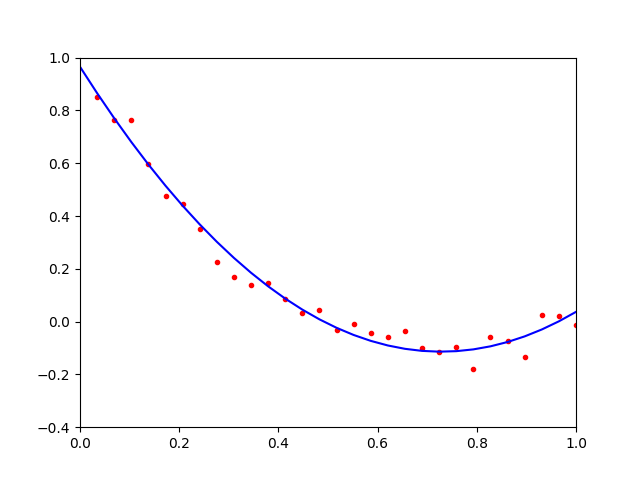
\includegraphics{problem_3_2_plot}


\begin{lstlisting}

import numpy as np
from matplotlib import pyplot as plt

x = np.linspace(0, 1, 30)
y = 2*x**2 - 3*x + 1 + 0.05*np.random.randn(*x.shape)

A = np.zeros((x.size, 3))
for i in range(A.shape[1]):
    A[:,i] = x**i

coefficients = np.linalg.lstsq(A, y, rcond=None)[0]

print("{0:1.4f} x^2 + {1:1.4f} x + {2:1.4f}".format(coefficients[2], coefficients[1], coefficients[0]))

plt.plot(x, y, 'r.', x, A @ coefficients, 'b')
plt.xlim([0, 1])
plt.ylim([-0.4, 1])
plt.show()

\end{lstlisting}



3) Beck Excercise 3.3. Write a function circle\_fit whose input is an $n \times m$ matrix
A, the columns of A are the m vectors in $\RR^n$ to which the circle should be fitted.
The call to the function will be of the form

(x, r) = circle\_fit(A)

Note: For this problem, report the output (x, r) for this set of points
and a plot of the circle together with the 5 points. Also submit a copy of the code
you used to solve the problem.

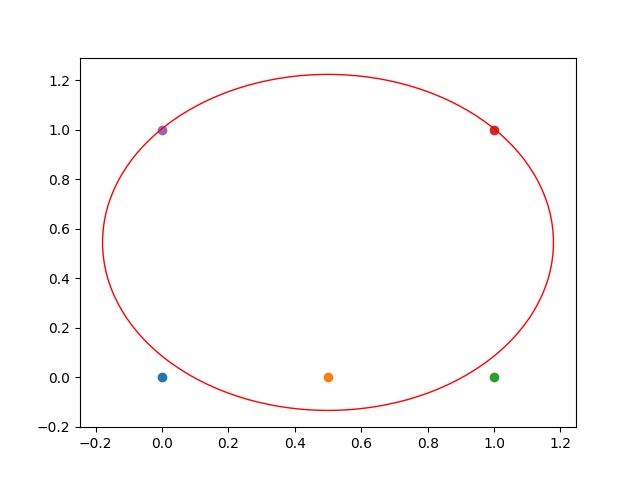
\includegraphics{problem_3_3_plot}

\begin{lstlisting}

from circle_fit import taubinSVD
import matplotlib.pyplot as plt

def circle_fit(points):
    xc, yc, r, sigma = taubinSVD(points)
    return ((xc, yc), r)

points = [[0, 0], [0.5, 0], [1, 0], [1, 1], [0, 1]]

(x, r) = circle_fit(points)


circle = plt.Circle(x, r, color='r', fill=False)

for point in points:
    plt.scatter(point[0], point[1])

plt.gca().add_patch(circle)

plt.show()

\end{lstlisting}


4) Beck Excercise 4.8. Let $f : \RR^n -> \RR$ be given by $f(x) = \sqrt{1 + ||x||^2}$.
Show that $f \in C_1^{1,1}$.

Hint: Show that $0 \leq u^T \nabla^2 f(x) u \leq ||u||^2$ $\forall u \in \RR^n$
and apply Theorem 4.20.


Theorem 4.20: Let $f \in C^2(\RR^n)$, the following are equivalent:

a) $f \in C_L^{1,1}(\RR^n)$

b) $||\nabla^2 f(x)|| \leq L$ $\forall x \in \RR^n$


\[\frac{d}{dx} (1 + ||x||^2)^{\frac{1}{2}}\]
\[= \frac{1}{2}(1+||x||^2)^{-\frac{1}{2}} \cdot 2x\]
\[= x \cdot (1 + ||x||^2)^{-\frac{1}{2}}\]

\[\frac{d}{dx} (x \cdot (1 + ||x||^2)^{-\frac{1}{2}})\]
\[= x \cdot \frac{d}{dx}((1 + ||x||^2)^{-\frac{1}{2}}) + \frac{d}{dx}(x) \cdot ((1 + ||x||^2)^{-\frac{1}{2}})\]
\[= x \cdot (-\frac{1}{2}(1 + ||x||^2)^{-\frac{3}{2}} \cdot 2x^T) + xx^T \cdot (1 + ||x||^2)^{-\frac{1}{2}}\]
\[= -(1 + ||x||^2)^{-\frac{3}{2}} \cdot xx^T + I_n \cdot (1 + ||x||^2)^{-\frac{1}{2}}\]

Let $a = (1 + ||x||^2)^{-\frac{1}{2}}$

\[= -a^3 xx^T + aI_n = aI_n - a^3xx^T\]


Show that: $0 \leq u^T (aI_n - a^3xx^T) u \leq ||u||^2$ $\forall u \in \RR^n$

\[\implies a u^T I_n u - a^3 u^T xx^T u\]
\[\implies a||u||^2 - a^3 u^T xx^T u\]
\[\implies a||u||^2 - a^3 ||u||^2 ||x||^2\]
\[\implies ||u||^2 (a - a^3 ||x||^2)\]

\[||u||^2 \geq ||u||^2 (a - a^3 ||x||^2) \geq 0\]
\[\implies 1 \geq a - a^3 ||x||^2 \geq 0\]
\[\implies 1 \geq (1 + ||x||^2)^{-\frac{1}{2}} - (1 + ||x||^2)^{-\frac{3}{2}} ||x||^2 \geq 0\]

Note that if $||x||$ is getting smaller, the hessian gets bigger.
Also, if $||x||$ is getting bigger, the hessian gets smaller.
Also, the norm is by definition $\geq 0$.


\[lim_{||x|| \to \infty} \frac{1}{\sqrt{1+||x||^2}} - \frac{||x||^2}{(1 + ||x||^2)^{\frac{3}{2}}}\]
\[\approx \frac{1}{\sqrt{||x||^2}} - \frac{||x||^2}{||x||^3}\]
\[\approx \frac{1}{||x||} - \frac{1}{||x||} = 0\]

The constants and whatnot don't matter since no matter what, you are ending up with
a higher power of $||x||$ in the denominator, which means
that term will always go to $0$ as $||x||$ gets large.


The smallest possible value of $||x||$ is $(0, 0)$.

Plugging it in gives:

\[\frac{1}{\sqrt{1 + 0}} - \frac{0}{0 + 1} = 1\]

So the min is $0$ and the max is $1$,
so the inequality holds and the function is in $C_1^{1,1}$.


5) Beck Excercise 5.2. Consider the Freudenstein and Roth test function

\[f(x) = f_1(x)^2 + f_2(x)^2, x \in \RR^2\]

where

\[f_1(x) = -13 + x_1 + ((5-x_2)x_2 - 2)x_2,\]
\[f_2(x) = -29 + x_1 + ((x_2 + 1)x_2 - 14)x_2.\]

i) Show that the function f has three stationary points. Find them and prove that
one is a global minimizer, one is a strict local minimum, and the third is a saddle point.



\includegraphics[scale=0.1]{problem_5_1}


\includegraphics[scale=0.1]{problem_5_2}


\includegraphics[scale=0.1]{problem_5_3}


\includegraphics[scale=0.1]{problem_5_4}


\includegraphics[scale=0.1]{problem_5_5}

Now we have to classify these 3 stationary points.


\[\frac{\partial^2 f}{\partial x_2^2} = 2(5 - 8x_2 + 6x_2 - 28) = 2(-3x_2 -23) = -6x_2 - 46\]

Evaluate $\frac{\partial^2 f}{\partial x_2^2}$ at the stationary points.


By looking at the sign, we get that:

(5, 4) is a saddle point

$\left( 15 + \frac{8}{3} \left( 1 + \sqrt{\frac{11}{2}} \right), \frac{2}{3} \left( 1 + \sqrt{\frac{11}{2}} \right) \right)$ is a local minimum.

$\left( 15 + \frac{8}{3} \left( 1 - \sqrt{\frac{11}{2}} \right), \frac{2}{3} \left( 1 - \sqrt{\frac{11}{2}} \right) \right)$ is a local minimum.

Plug into $f(x)$ to find out which is the global minimizer.

If we plug this into a calculator,
we find that that he first local minimum
gives $\approx 148.71$ and the second local minimum gives $\approx 277.44$.

That means that the global minimizer is:

\[\left( 15 + \frac{8}{3} \left( 1 + \sqrt{\frac{11}{2}} \right), \frac{2}{3} \left( 1 + \sqrt{\frac{11}{2}} \right) \right)\]

since $148.71 < 277.44$.



ii) Use Python to employ the following three methods on the problem of minimizing f:

a) the gradient method with backtracking and parameters $(s, \alpha, \beta) = (1, 0.5, 0.5)$.

b) the hybrid Newton's method with parameters $(\alpha, \beta) = (0.5, 0.5)$

c) the damped Gauss-Newton method with a backtracking line search strategy with
parameters $(s, \alpha, \beta) = (1, 0.5, 0.5).$

All the algorithms should use the stopping criteria $||\nabla f(x)|| \leq 10^{-5}$.
Each algorithm should be employed four times on the following four starting points:
$(-50, 7)^T, (20, 7)^T, (20, -18)^T,$ and $(5, -10)^T$. For each of the four starting
points, compare the number of iterations and point to which each method converged.
If a method did not coverge, explain why.

Note: For this problem, additionally submit a copy of
the code you used to solve the problem.


6) Beck Excercise 5.3. Let f be a twice continuously differentiable function
satisfying $L I_n \succeq \nabla^2 f(x) \succeq m I_n$ for some
$L > m > 0$ and let $x^{*}$ be the unique minimizer of f over $\RR^n$.

i) Show that

\[f(x) - f(x^{*}) \geq \frac{m}{2} ||x - x^{*}||^2\]

for any $x \in \RR^n$.


First, the second order taylor expansion of f around $x^{*}$ is:

\[f(x) \approx f(x^{*}) + \nabla f(x^{*})^T (x - x^{*}) + \frac{1}{2} (x - x^{*})^T \nabla^2 f(G)(x - x^{*})\]

for some $G$ in the line segment $[x, x^{*}]$.


Since $x^{*}$ is the minimizer of f, $\nabla f(x^{*}) = 0$, so

$f(x) \approx f(x^{*}) + \frac{1}{2} (x - x^{*})^T \nabla^2 f(L) (x - x^{*})$


By the definition, $\nabla^2 f(G)$ is positive definite and the smallest eigenvalue $\geq m$.

So,


\[(x - x^{*})^T \nabla f((G) (x - x^{*})) \geq m ||x - x^{*}||^2\]

Substituting this back into our taylor expansion gives:

\[f(x) \geq f(x^{*}) + \frac{m}{2} ||x - x^{*}||^2\]

\[\implies f(x) - f(x^{*}) \geq \frac{m}{2} ||x - x^{*}||^2\]

for any $x \in \RR^n$.


ii) Let $\{x_k\}_{k \geq 0}$ be the sequence generated by the damped Newton's
method with constant step-size $t_k = \frac{m}{L}$. Show that

\[f(x_k) - f(x_{k+1}) \geq \frac{m}{2L} \nabla f(x_k)^T (\nabla^2 f(x_k))^{-1} \nabla f(x_k).\]

for any $x \in \RR^n$.


Damped Newton's method:

\[x_{k+1} = x_k - t_k (\nabla^2 f(x_k))^{-1} \nabla f(x_k)\]

With $t_k = \frac{m}{L}$, we have:

\[x_{k+1} = x_k - \frac{m}{L}(\nabla^2 f(x_k))^{-1} \nabla f(x_k)\]

Let $\lambda_k^2 = \nabla f(x_k)^T (\nabla^2 f(x_k))^{-1} \nabla f(x_k)$

Goal:

\[f(x_k) - f(x_{k+1}) \geq \frac{m}{2L} \lambda_k^2\]


Quadratic taylor approximation of f around $x_k$:

\[f(y) \approx f(x_k) + \nabla f(x_k)^T (y - x_k) + \frac{1}{2} (y - x_k)^T \nabla^2 f(x_k) (y - x_k)\]

Let $y = x_{k+1}$. We then get:

\[f(x_{k+1}) \approx f(x_k) + \nabla f(x_k)^T ((x_k - \frac{m}{L}(\nabla^2 f(x_k))^{-1} \nabla f(x_k)) - x_k) + \frac{1}{2} ((x_k - \frac{m}{L}(\nabla^2 f(x_k))^{-1} \nabla f(x_k)) - x_k)^T \nabla^2 f(x_k) ((x_k - \frac{m}{L}(\nabla^2 f(x_k))^{-1} \nabla f(x_k)) - x_k)\]

Simplification:

\[f(x_{k+1}) \approx f(x_k) - \frac{m}{L} \nabla f(x_k)^T (\nabla^2 f(x_k))^{-1} \nabla f(x_k) + \frac{m^2}{2L^2} \nabla f(x_k)^T (\nabla^2 f(x_k))^{-1} \nabla^2 f(x_k) (\nabla^2 f(x_k))^{-1} \nabla f(x_k)\]

Since $\nabla^2 f(x)$ is positive definite, we can simplify this to:

\[\frac{m^2}{2L^2} \nabla f(x_k)^T (\nabla^2 f(x_k))^{-1} \nabla f(x_k) \leq \frac{m}{2L} \nabla f(x_k)^T (\nabla^2 f(x_k))^{-1} \nabla f(x_k)\]

We can deduce from this that:

\[f(x_k) - f(x_{k+1}) \geq \frac{m}{2L} \nabla f(x_k)^T (\nabla^2 f(x_k))^{-1} \nabla f(x_k)\]



iii) Show that $x_k \to x^{*}$ as $k \to \infty$.


Combining the inequalities from i and ii, we get:

\[f(x_{k+1}) \leq f(x_k) - \frac{m}{2L} \nabla f(x_k)^T (\nabla^2 f(x_k))^{-1} \nabla f(x_k)\]

$x^{*}$ is the global minimizer, so f is bounded below by $f(x^{*})$.
This means that $f(x_k)$ is decreasing and bounded below by $f(x^{*})$.
So, $f(x_k)$ converges to some value G.

This implies that $f(x_k) - f(x_{k+1})$ approaches 0 as $k \to \infty$.

Now, from our inequality,

\[\nabla f(x_k)^T (\nabla^2 f(x_k))^{-1} \nabla f(x_k) \to 0\]

as $k \to \infty$.


Because $\nabla^2 f(x)$ is positive definite and $\leq L$ and $\geq m$, that means that

\[\nabla f(x_k) \to 0\]

as $k \to \infty$.

But $\nabla f(x_k)$ is only 0 at $x^{*}$,
so $x_k \to x^{*}$

as $k \to \infty$.


\end{document}
